\documentclass[10pt, compress]{beamer} 
\usetheme{m}

\usepackage{booktabs}
\usepackage[scale=2]{ccicons}
\usepackage{minted}
\usepackage[style=english]{csquotes}

\usepackage[round]{natbib}

\hypersetup{
    colorlinks=true,       % false: boxed links; true: colored links
    linkcolor=black,          % color of internal links
    citecolor=black,        % color of links to bibliography
    filecolor=magenta,      % color of file links
    urlcolor=black           % color of external links
}

\urlstyle{same}

\usemintedstyle{trac}

\title{System Architecture}
\subtitle{A (hopefully) gentle introduction}
\date{\today}
\author{Andres Kütt}
\institute{Riigi Infosüsteemi Amet}


\begin{document}

\maketitle

\section{Introduction}
\begin{frame}[fragile]
  \frametitle{Agenda today}
\begin{itemize}
	\item Intro. Importance of the topic. Global challenges. Conventional assumptions
	\item System thinking. Concept of value
	\item Form, Function, Concept intro. Examples
	\item Identify the entities of the system and their function
	\item Exercise: Form, function and concept of a country
	\item Relationships among entities. Feedback, emergence
	\item Introduction to complexity
	\item System thinking and architecture in public sector
	\item Role of a software architect
\end{itemize}
	
\end{frame}

\begin{frame}[fragile]
	\frametitle{Andres Kütt}
	\begin{columns}[t]
		\begin{column}{7cm}
			\begin{itemize}
				\item Building software for living since 1993
				\item In architect-like roles for the past 10 years
				\item $\approx$MSc (UT, Statistika), MBA (EBS), MSc (MIT)
				\item Currently architect of Estonian Information System
				\item Skype, Hansapank, EMTA etc. in the past
				\item Some teaching experience
			\end{itemize}
		\end{column}
		\begin{column}[T]{3cm}
			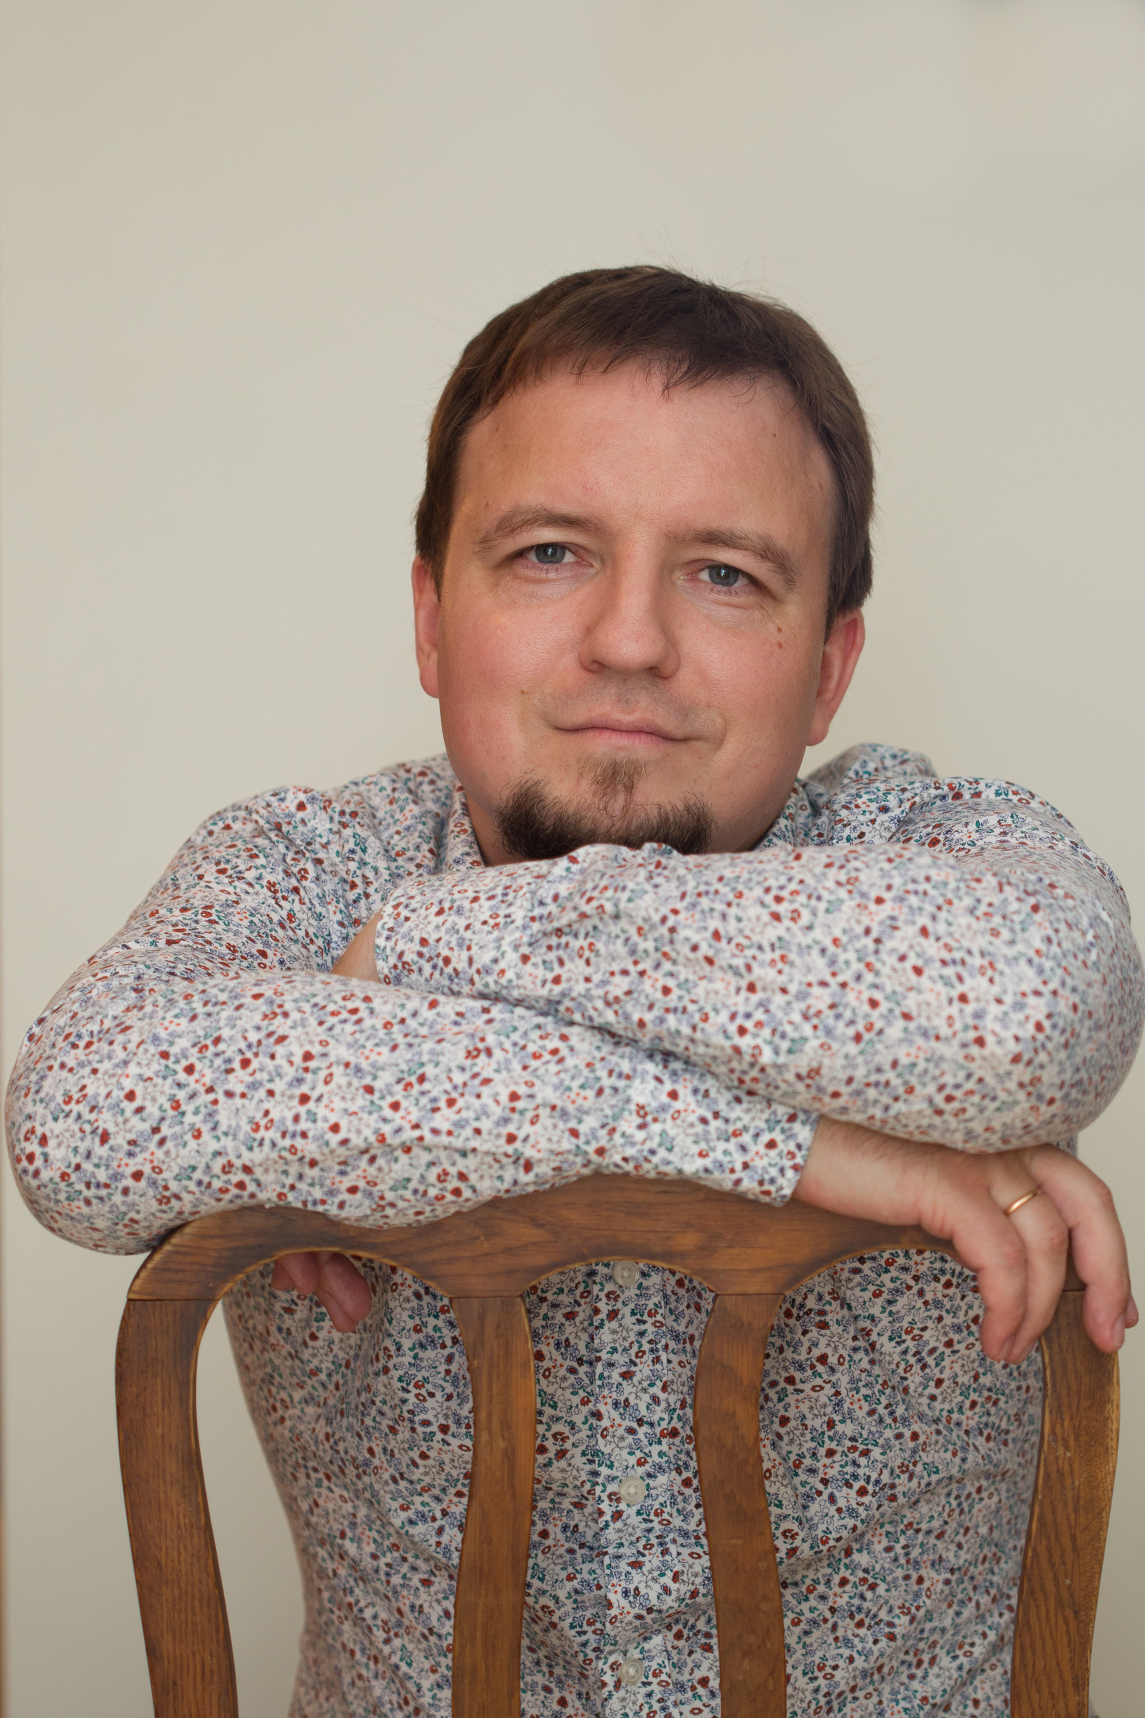
\includegraphics[width=\textwidth]{author.jpg}
		\end{column}
	\end{columns}
\end{frame}

\begin{frame}[fragile]
  \frametitle{Structure of today}
	\begin{itemize}
		\item Two main sections
			\begin{itemize}
				\item Fundamentals of system architecture
				\item Theoretical foundations of public sector architecture
			\end{itemize}
		\item Nine 30-minute blocks of study punctuated by two breaks
		\item Each block but one contains 
			\begin{itemize}
				\item 20 minutes of slides, 
				\item 5 minutes of paired discussion
				\item 5 minutes of common discussion
			\end{itemize}
		\item The questions on paired discussion form the basis of grading
		\item The 5th block is different consisting of a team exercise followed by discussion
	\end{itemize}
\end{frame}

\begin{frame}[fragile]
  \frametitle{The contents}
	\begin{itemize}
		\item The theory is mainly based on \cite{crawley2015systems} and various lectures by prof. Crawley
		\item The goal is to talk about architecture in general not software architecture in particular
		\item Have patience: it is really hard to that much into 4.5 hours without your heads exploding. Certain things will not make immediate sense
	\end{itemize}
\end{frame}

\section{Fundamentals of system architecture}
\begin{frame}[fragile]
  \begin{quote}
    Architecture is an abstract description of the entities of a system and the relationships between those entities. It can be seen as a set of decisions. 
  \end{quote}
	\cite{crawley2015systems}
\end{frame}

\begin{frame}[fragile]
  \frametitle{Properties of architecture}
	\begin{itemize}
		\item Architecture can either emerge from a development process or be explicit
		\begin{itemize}
			\item Everything has an architecture
			\item Explicit architecture provides more (but not ultimate) control
		\end{itemize}
		\item It is about decision quality under the conditions of ambiguity
		\begin{itemize}
			\item Small improvements here can lead to a lot of benefit down the line
		\end{itemize}
		\item In software, architecture is an outcome of a continuous process not a one-time activity
		\begin{itemize}
			\item Design decisions need to be made constantly as the systems evolve
		\end{itemize}
	\end{itemize}
\end{frame}

\begin{frame}[fragile]
  \frametitle{Benefits of good architecture}
  
  What do we generally want from a system? 
  
  \begin{itemize}
  	\item Meet shareholder needs 
	\item Deliver value
	\item Integrate easily
	\item Evolve flexibly
	\item Operate simply and reliably
  \end{itemize}
  
	Explicitly developed architecture allows us to have a measure of control over all this
\end{frame}

\begin{frame}[fragile]
  \frametitle{Conventional assumptions about organisations}
  \begin{itemize}
  	\item They are culturally, technically etc. homogenous
	\begin{itemize}
		\item \enquote{You and your architecutre can get stuffed, I know better what works locally} (a random person from Montevideo)
	\end{itemize}
	\item Organisational and legal borders are clearly defined 
	\begin{itemize}
		\item Tightly integrated supply chains
		\item Global organisations partnering with each other largely ignoring states
	\end{itemize}

	\item Relative independence from global challenges
	\begin{itemize}
		\item Many things need to be resolved within next decades. You are either part of the solution or you are part of the problem
	\end{itemize}

	\item Controlled and contained IT
	\begin{itemize}
		\item Specialised hw/software package operated by highly trained employees vs. general purpose soft- and hardware all over the place
	\end{itemize}
	
  \end{itemize}
  
\end{frame}

\begin{frame}[fragile]
  \frametitle{The challenge}
  
  As the assumptions no longer hold, we are faced with:
  \begin{itemize}
		\item Higher complexity both within the organisation and globally
		\item Higher levels of upstream uncertainty
		\item No way to separate IT from the rest of the organisation without loss of fidelity
  \end{itemize}
  
  \begin{center}
  	\textbf{We need to figure out a better way to provide \\the benefits of good architecture}
  \end{center}
\end{frame}

\begin{frame}[fragile]
  
  \begin{center}
  	\textbf{This is not about architecture astronautics\\[4mm] \large{What we discuss today is to be applied to \\make better stuff every single day}}
  \end{center}
\end{frame}


%Arutelu koht
\begin{frame}[fragile]
  \frametitle{Discussion}
		\begin{center}
			\textbf{What do you want to get out of today?}
		\end{center}
\end{frame}
%Arutelu koht

\section{System thinking basics}
\begin{frame}[fragile]
	\begin{center}
		\begin{quote}
			A system is a set of entities and their relationships, whose functionality is greater than the sum of the individual entities
		\end{quote}
	\end{center}
		\cite{crawley2015systems}
\end{frame}


\begin{frame}[fragile]
  \frametitle{System thinking definition}
  System thinking is not about thinking systematically
  	\begin{itemize}
  		\item It is about thinking about a question, circumstance, or problem explicitly as a system
		\begin{itemize}
			\item Observe, how we make no assumptions about the nature of the entities
			\item Emergence of new functions is a key part of the definition. This is what allows systems to generate value
		\end{itemize}
		\item System thinking is a way of thinking
		\begin{itemize}
			\item Therefore, it is not a science or a theory
			\item It is a mental model
			\item All models are wrong but some models are useful \citep{box1976science}
			\item It should be used alongside with other modes of thinking and logical reasoning 
		\end{itemize}		
	\end{itemize}
\end{frame}

\begin{frame}[fragile]
  \frametitle{Examples of systems}
  	\begin{itemize}
  		\item Sand and a funnel combined yield the function of timekeeping
		\begin{itemize}
			\item Neither the funnel alone nor sand can do that
			\item But also, a function of triggering a trap can emerge
		\end{itemize}
		\item A particular group of people combined can yield the function of winning football matches
		\begin{itemize}
			\item In addition to function, performance emerges
			\item Performance is an attribute of the emergent function
		\end{itemize}		
		\item A set of mechanical and chemical components can be combined to result in a car
		\begin{itemize}
			\item A group of \enquote{-ilities} - reliability, operability, respectability etc. - emerges
			\item Safety is one of these
			\item Note that in this model, usability is an emergent property of the system 
		\end{itemize}		
		
	\end{itemize}
\end{frame}

\begin{frame}[fragile]
  \frametitle{Emergence of emergencies}
  	Not all emergency is desirable
  	\begin{itemize}
  		\item In December of 1984, 40 tons of methyl isocyanate was released to atmosphere at a chemical plant in Bhopal, India
		\begin{itemize}
			\item Worst industrial accident in history 
			\item 2 000 fatalities, 200 000 injuries, 10 000 permanent disabilities \citep[conservative estimates]{leveson2011engineering}
		\end{itemize}
		\item A \textit{bona fide} systemic failure
		\begin{itemize}
			\item Unclear job descriptions
			\item Inadequately planned safety measures
			\item Human error
			\item Business error in decreasing safety to save cost
		\end{itemize}
		\item The same principle applies to information securty
		\begin{itemize}
			\item Security is an emergent behavior of a system
			\item Cannot thus be fully predicted, only designed for
		\end{itemize}
	\end{itemize}
\end{frame}

\begin{frame}[fragile]
  \frametitle{Emergence and value}
  	How exactly do systems generate value?
		\begin{itemize}
			\item This is how the work of an architect is justified
			\begin{itemize}
				\item A well-architected system \emph{might} generate more value
			\end{itemize}
			\item Benefit stems from 
			\begin{itemize}
				\item The system performing the intended function with intended performance
				\item All the ilities being there 
				\item Lack of emergencies
				\item Basically, the emergence happening in a desired way
			\end{itemize}
			\item The concept of benefit implies existence of a user, as benefit is always relative
			\item Value is defined as  \textbf{benefit at cost}
			\begin{itemize}
				\item All artificially constructed systems incur a cost
			\end{itemize}
		\end{itemize}
\end{frame}


\begin{frame}[fragile]
  \frametitle{Key questions of systems thinking}
	These questions should be asked when thinking about a system
		\begin{enumerate}
			\item What is the system made of?
			\begin{itemize}
				\item Again transcending discipline boundaries
			\end{itemize}
			\item What is \emph{the particular} mental model of the system?
			\begin{itemize}
				\item Remember the one about all models being wrong? 
				\item Many are applicable, which one is the most useful at the moment?
			\end{itemize}

			\item Where are the system boundaries?
			\begin{itemize}
				\item Everything is interconnected, where do we draw the line?
			\end{itemize}

			\item What is the system context?
			\begin{itemize}
				\item What interfaces do we need to keep in mind?
			\end{itemize}

		\end{enumerate}
\end{frame}



%Arutelu koht
\begin{frame}[fragile]
  \frametitle{Discussion}
		\begin{center}
			\textbf{What is architecture?}
		\end{center}
\end{frame}
%Arutelu koht

\begin{frame}[fragile]
  \frametitle{Answering question 1: what is the system made of?}
	
  	\begin{itemize}
		\item This is where you define subject of your architecture
		\begin{itemize}
			\item Do we get hardware involved?
			\item How about people? (NB! people are \emph{hard}) 
		\end{itemize}
		\item There is no such thing as a green field, you are always working with an existing system
		\begin{itemize}
			\item At the very least the users are there
			\item It is also beneficial to re-visit this question as the system evolves
		\end{itemize}
	\end{itemize}
\end{frame}

\begin{frame}[fragile]
  \frametitle{The steps}
	Steps to answering \enquote{what the system is made of?}:
		\begin{enumerate}
			\item Identify form and function
			\item Identify entities of the system and their form and function
			\item Identify the relationships
			\item Predict emergence
		\end{enumerate}
		
\end{frame}

\begin{frame}[fragile]
  \frametitle{Step 1. Identify form and function}
  \begin{itemize}
  	\item Form is what the system \emph{is}
	\begin{itemize}
		\item form is stable over a period of time
		\item form is the part of the system that is made or assembled
	\end{itemize}
	\item Function is what the system \emph{does}
	\begin{itemize}
		\item function is what causes performance and ilities
		\item this is why the system exists or is employed
		\item emergence occurs in the function domain
		\item function consists of a process and an operand: something (operand) changes state as the system does something (process)
	\end{itemize}
  \end{itemize}
	
	
\end{frame}


\begin{frame}[fragile]
  \frametitle{Examples of form and function}
  \begin{itemize}
  	\item An amplifier
	\begin{itemize}
		\item form is the wires, transistors and resistors
		\item functions is amplification (process) of a signal (operand)
	\end{itemize}
	\item Circulatory system
	\begin{itemize}
		\item form is heart, lungs, capillaries
		\item function is transporting (process) oxygen (operand)
	\end{itemize}
	\item Project team
	\begin{itemize}
		\item form is the team members
		\item function is delivering (process) result (operand)
	\end{itemize}

  \end{itemize}
	
\end{frame}

\begin{frame}[fragile]
  \frametitle{Form and function. Observations}
  \begin{itemize}
  	\item Both can only be expressed via an abstract model
	\begin{itemize}
		\item Software, as opposed to physical things, cannot be experienced directly
		\item It is thus vital the abstract model is as useful and unambiguous as possible 
	\end{itemize}
	\item The same function can be performed by several sets of form elements and vice versa
	\begin{itemize}
		\item Therefore we need a third notion, \textbf{the concept}, creating a one-to-one mapping
		\item These mappings are not equivalent 
		\item I am yet to see a useful representation of this relating functional and form models
	\end{itemize}
  \end{itemize}
	
\end{frame}

\begin{frame}[fragile]
  \frametitle{Form and function. More observations}
  \begin{itemize}
  	\item It is much more difficult to do for some systems than for others
	\begin{itemize}
		\item Physical things are much easier than abstract concepts like software
		\item Form of an ice sculpture. Is oxygen in the water part of the form?
		\item What is the Internet actually made of?
	\end{itemize}
	\item There is a tendency to get carried away with form
	\begin{itemize}
		\item Where does the system end?
		\item Is IETF part of the Internet? What about sysadmins of the core DNS boxes?
		\item In the universe, everything is interconnected
	\end{itemize}
  \end{itemize}
	
\end{frame}

%Arutelu koht
\begin{frame}[fragile]
  \frametitle{Discussion}
		\begin{center}
			\textbf{Where does concept of a system come from?}
		\end{center}
\end{frame}
%Arutelu koht

\begin{frame}[fragile]
  \frametitle{The steps}
	Steps to answering \enquote{what the system is made of?}:
		\begin{enumerate}
			\item Identify form and function
			\item \textbf{Identify entities of the system and their form and function}
			\item Identify the relationships
			\item Predict emergence
		\end{enumerate}
		
\end{frame}


\begin{frame}[fragile]
	\frametitle{Step 2. Identify the entities of the system and their function}
		
	What is the structure of form and function of our system?
	
	\begin{enumerate}
		\item Include everything you feel is important
		\item Throw out everything that turns out not to be 
		\item See what can be generalised and clumped together
		\item Define boundaries and interfaces
		\item Repeat unless the result is both useful and manageable
	\end{enumerate}
	
	The basic algorithm:
	\center{\textbf{Keep adding and removing things until you like the result}}
	
\end{frame}

\begin{frame}[fragile]
	\frametitle{On adding and removing things}
	
	Think holistically
	\begin{itemize}
		\item Add people, technology, hardware, software, everything important-looking
		\item Be aware of unknown-unknowns: things you do not know you do not know. 
		\begin{itemize}
			\item For software folks this is often people
			\item For legal folks, this is often anything related to real life
		\end{itemize}
	\end{itemize}
	
	Focus
	\begin{itemize}
		\item The $7\pm2$ rule. There is a limit to human cognition \citep{miller1956magical}
		\item "Is the entity important in determining the outcome and the emergence that I am interested in?"
	\end{itemize}
\end{frame}

\begin{frame}[fragile]
	\frametitle{Two key types of clumping}
	\begin{description}
		\item[Abstraction] Replace instances with class. \enquote{Employee} instead of Alice, Bob and Charlie
		\item[Modularisation] What things relate to each other more than to others?
		\begin{itemize}
			\item Footnote: there are great tools for doing that algorithmically. See \cite{browning2001applying}
		\end{itemize}
	\end{description}
\end{frame}

\begin{frame}[fragile]
	
	\frametitle{Guidelines for creating abstractions and modules}
		\begin{itemize}
			\item Conceal the unimportant and expose the important
			\begin{itemize}
				\item On system level, exact class structure might not be relevant but the interface probably is
			\end{itemize}
			\item Make sure appropriate relationships are retained
			\begin{itemize}
				\item Team members might cooperate a lot even if teams themselves do not
			\end{itemize}
			\item Create abstractions at the right level of decomposition or aggregation
			\begin{itemize}
				\item \enquote{Screw} is a pretty useless abstraction
			\end{itemize}
			\item Simplify, until you notice loss of fidelity, and no further
			\begin{itemize}
				\item \enquote{Software running on hardware being used by a user} is a valid but not useful model 
			\end{itemize}
		\end{itemize}

\end{frame}

\begin{frame}[fragile]
	
	\frametitle{Define system boundaries}

\begin{quote}
God, grant me the serenity to accept the things I cannot change, the courage to change the things I can, and the wisdom to know the difference
\end{quote}
	
	\begin{itemize}
		\item \emph{Choose} system boundary in a way that is useful
		\item By defining system boundaries, you define interfaces: the relationships crossing the system boundary
		\item Cleary differentiate between
		\begin{itemize}
			\item Things you can change
			\item Things that make up a system
		\end{itemize}
		\item These two very seldom overlap
		\begin{itemize}
			\item Ignore the big picture and get a useless system
			\item Try to change the big picture and get a bloody nose
		\end{itemize}
		
	\end{itemize}

\end{frame}

\begin{frame}[fragile]
	\frametitle{Stop condition}
	
	All steps alter the results of previous steps, so there's a cycle. When do you stop?
	\begin{itemize}
		\item Do all entities contribute to the function and emergence you are interested in?
		\item Is there an element of form contributing to each function?
		\item Can you explain the system on a single sheet of paper?
		\item Is the result useful?
	\end{itemize}
\end{frame}

%Arutelu koht
\begin{frame}[fragile]
  \frametitle{Discussion}
		\begin{center}
			\textbf{What if the resulting system is too complex?}
		\end{center}
\end{frame}
%Arutelu koht


\begin{frame}[fragile]
  \frametitle{Exercise: form function and concept of a country}
  	\begin{itemize}
		\item Go through first two steps of system analysis for a country of your choosing
		\begin{itemize}
			\item Identify form and function
			\item Identify entities of the system and their form and function
		\end{itemize}
		\item Present the results
	\end{itemize}
\end{frame}


\begin{frame}[fragile]
  \frametitle{The steps}
	Steps to answering \enquote{what the system is made of?}:
		\begin{enumerate}
			\item Identify form and function
			\item Identify entities of the system and their form and function
			\item \textbf{Identify the relationships}
			\item Predict emergence
		\end{enumerate}
		
\end{frame}

\begin{frame}
	\frametitle{Step 3. Relationships among entities}
	Functional relationships \emph{do} something, they are dynamic in nature
	\begin{itemize}
		\item operands are exchanged or acted upon
		\item sometimes called \textbf{interactions}
		\item a heart exchanges blood with a lung
	\end{itemize}
	Formal relationships are relationships that \emph{exist}, they are static
	\begin{itemize}
		\item these relationships exist stably for some period of time
		\item usually a connection or a geometric relationship
		\item a class is within a package
		\item sometimes called \textbf{structure}
	\end{itemize}
	
	Typically, (but much less in software), a formal relationship is required for a functional relationship
\end{frame}

\begin{frame}
	\frametitle{Representing relationships}
	\begin{center}
	The same system represented in two ways:\\[4mm]
	\begin{columns}[T]
		\begin{column}{4cm}
			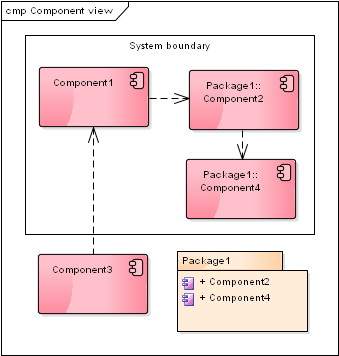
\includegraphics[height=4cm]{component.png}\\
			A standard UML component diagram
		\end{column}
		\begin{column}[T]{4cm}
			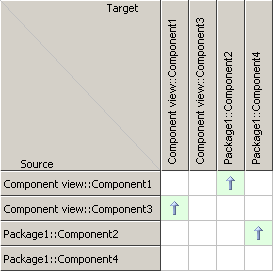
\includegraphics[height=4cm]{matrix.png}\\
			A DSM (see \cite{browning2001applying} for details)
		\end{column}
	\end{columns}
	\end{center}
\end{frame}

\begin{frame}
	\frametitle{Step 4. Emergence}
	Emergence is why we study systems in the first place
	\begin{itemize}
		\item Firmly in the functional domain, form leads to function that leads to emergence
		\begin{itemize}
			\item It is about how the elements are put together
			\item The elements themselves are important but architecture leads to emergence 
		\end{itemize}
		\item Cannot be fully predicted or controlled by definition
		\item Information/Cyber security and safety are emergent properties of a system
		\begin{itemize}
			\item Understanding how emergence works is thus crucial
			\item Since emergence stems from architecture, so do security and safety
		\end{itemize}
	\end{itemize}
\end{frame}

\begin{frame}
	\frametitle{Predicting emergence}
	This is the crux of system thinking \\
	\begin{description}
		\item[Precedent] We have experience and thus know, what shall happen
		\item[Experiment] We can build an experiment to see, what shall happen
		\item[Model] We can build a model to simulate, what shall happen
	\end{description}
	
	\begin{itemize}
		\item Many modern systems are new, too large to do experiments for and too complex to model
		\item These we can reason about using system thinking or other frameworks
	\end{itemize}
\end{frame}

%Arutelu koht
\begin{frame}[fragile]
  \frametitle{Discussion}
		\begin{center}
			\textbf{Can we talk about emergence in legal systems?}
		\end{center}
\end{frame}
%Arutelu koht

\begin{frame}
	\frametitle{Defining complexity}
		There are many definitions, \cite{mitchell2009complexity} brings examples. Complexity as \ldots
	
		\begin{itemize}
			\item \ldots size. Function of the number of elements and their relationships
			\item \ldots (Shannon) entropy. Information content of the system
			\item \ldots algorithmic information content. Compressability
			\item \ldots logical or thermodynamic depth. The cost of construction
			\item \ldots relationship between input and output. Predictability 
			\item \ldots fractal dimension
	\end{itemize}

\end{frame}

\begin{frame}
	\frametitle{More about complexity}
	\begin{itemize}
		\item Complexity is an emergent property of a system and therefore a general concept
		\item The arithmetical definition yields most practical tools
		\begin{itemize}
			\item Counting things is easy
			\item Limited in usefulness because of its static nature
		\end{itemize}
		\item Complexity vs. complicatedness
		\begin{itemize}
			\item Complicatedness is the extent to which a system appears complex
		\end{itemize}
		\item Static vs. dynamic complexity
		\begin{itemize}
			\item Dynamic complexity is the ability of a system to exhibit complex behaviour over time
			\item Static complexity stems from formal relationships, dynamic complexity from functional ones
		\end{itemize}
	\end{itemize}
\end{frame}

\begin{frame}
	\frametitle{Exponential nature of complexity}
	\begin{center}
		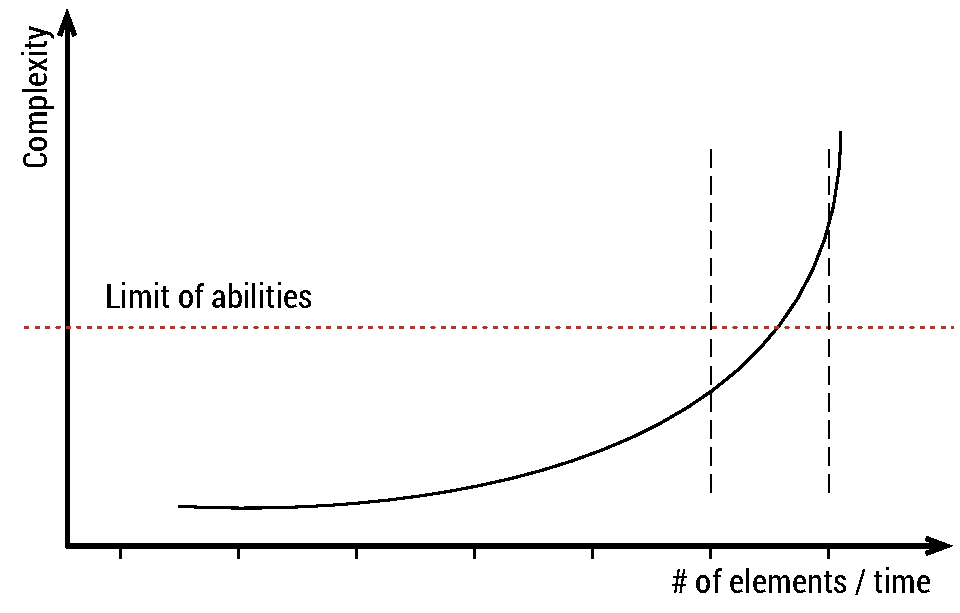
\includegraphics[width=.8\textwidth]{exp_complex.pdf}\\[3mm]
	Complexity seems to have a tendency to increase exponentially
	\end{center}

\end{frame}

\begin{frame}
	\frametitle{Implications of this}
	
	This is why complexity needs to be actively managed. There are three basic strategies
	\begin{description}
		\item[Flatten the curve] Working on the system should add the least amount of complexity possible. Engineering.
		\item[Stop moving] Stop adding features, growing the org. etc. This is what eventually happens. Management. 
		\item[Raise the capabilities] Increase the ability of an organisation to cope. Dynamic capabilities.
	\end{description}
\end{frame}

%Arutelu koht
\begin{frame}[fragile]
  \frametitle{Discussion}
		\begin{center}
			\textbf{How to assess complexity of a set of laws?}
		\end{center}
\end{frame}
%Arutelu koht


\section{Foundations of public sector architecture}
\begin{frame}[fragile]
	\frametitle{Know and respect your context}
		\begin{columns}[T]
		\begin{column}{7.5cm}
			\begin{itemize}
				\item Understand dependencies between layers
				\item Know your limits (i.e. define boundaries carefully)
				\item Learn to accept what you cannot change
				\item Maintain alignment between layers
				\item Build horizontal and vertical relationships
				\item Ponder the source and impact of changes
			\end{itemize}
		\end{column}
		\begin{column}[T]{3.5cm}
			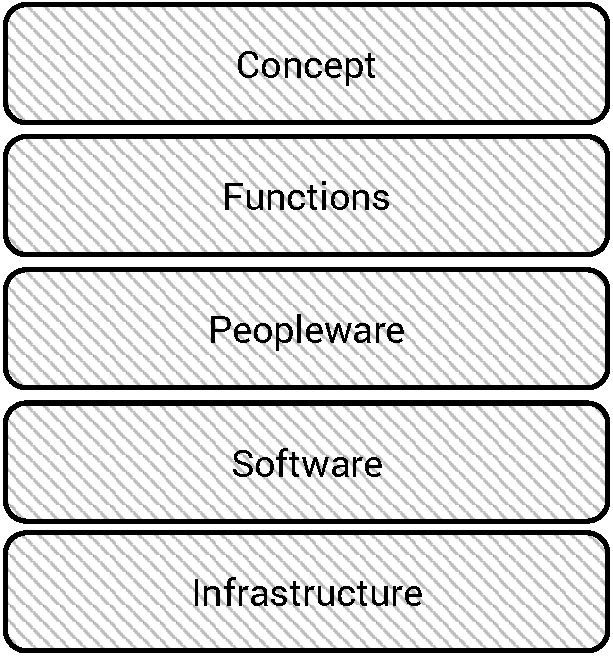
\includegraphics[width=\textwidth]{govlayers.pdf}
		\end{column}
	\end{columns}

\end{frame}

\begin{frame}[fragile]
	\frametitle{On legal issues}
		\begin{columns}[T]
		\begin{column}{7.2cm}
			\begin{itemize}
				\item In public setting, the top layers a held together by a legal framework, usually subject to democratic process
				\item The bottom layers are held together by open source and the internet
				\item The former is local, the latter is global
				\item This creates a barrier to change
			\end{itemize}
		\end{column}
		\begin{column}[T]{3.8cm}
			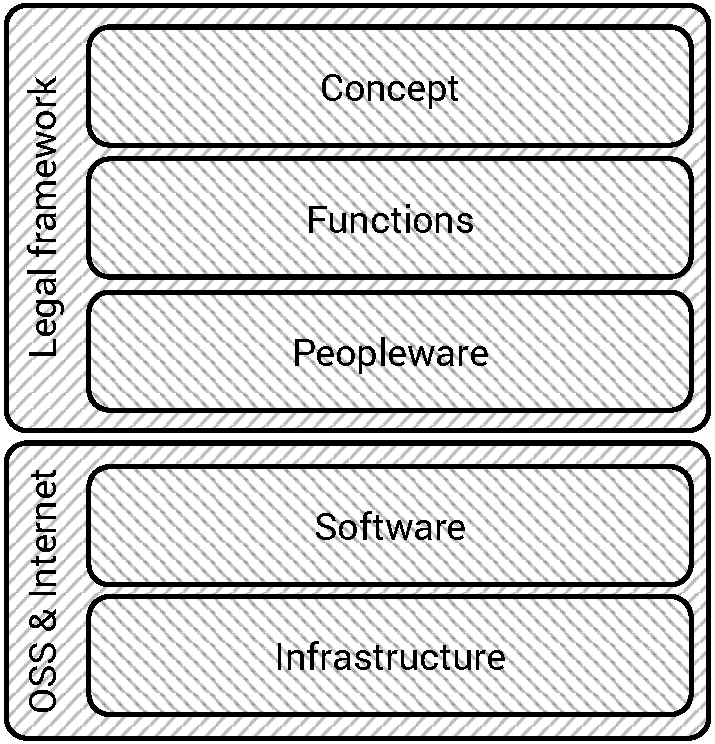
\includegraphics[width=\textwidth]{govlayers_legal.pdf}
		\end{column}
	\end{columns}
\end{frame}

\begin{frame}[fragile]
	\frametitle{Peculiarities of public sector}
	\begin{itemize}
		\item There is no profit
		\begin{itemize}
			\item Taxes are collected to provide public services
			\item If these are not spent, the customer is not getting their moneys worth
			\item Therefore, there is no intrinsic efficiency pressure
		\end{itemize}
		\item You can't risk to break the law
		\begin{itemize}
			\item In private sector, you can accept any risk 
			\item In public sector, one \emph{cannot} accept the risk of breaking the law
			\begin{itemize}
				\item At least this is my understanding as an engineer
				\item E.g. you can't put encrypted personal data of citizens to a public cloud as breaking the crypto in the future is a real risk that would lead to exposing personal data
			\end{itemize} 
		\end{itemize}
	\end{itemize}
\end{frame}

%Arutelu koht
\begin{frame}[fragile]
  \frametitle{Discussion}
		\begin{center}
			\textbf{How to express legal architecture?}
		\end{center}
\end{frame}
%Arutelu koht


\begin{frame}[fragile]
  \frametitle{Role of a software architect in government setting}
  	\begin{itemize}
		\item Manage, control and own complexity
		\item Prevent lock-in
		\item Build bridges
		\item Predict emergence
	\end{itemize}
\end{frame}

\begin{frame}[fragile]
	\frametitle{Manage, control and own complexity}
	
	\begin{itemize}
		\item Do not forget complicatedness!
		\item Everybody else is interested in more of it
		\begin{itemize}
			\item Bureaucrats do not mind complex processes seeking to control reality
			\item Engineers love to engineer
			\item Project managers have deadlines and budgets
			\item Entropy tends to increase
		\end{itemize}
		\item Complexity has the property of being complex
		\begin{itemize}
			\item Once the threshold is breached, backing down might be impossible
			\item But it would be considered the job of an architect
			\item Thus, constant effort is required to keep system complexity manageable
		\end{itemize}
		\item Complexity needs to be represented at decisions
		\begin{itemize}
			\item Governments love waterfall but less and less problems are simple enough to be solved using it
			\item Legal, business and organisational design decisions are good examples
		\end{itemize}		
	\end{itemize}
\end{frame}

\begin{frame}[fragile]
	\frametitle{Prevent lock-in}

	\begin{itemize}
		\item In private sector, IP governance can prevent lock-in
		\item In public sector, there is no concept of IP and thus lock-in can happen more easily
		\item How lock-in occurs
		\begin{itemize}
			\item Vendor develop architecture embedding their concept in the process
			\item Every new vendor has to learn and adapt to the the mental models of the original vendors, which is costly
		\end{itemize}
		\item Architect can actively drive concept development
		\begin{itemize}
			\item Now all vendors have the same barrier of entry
			\item And therefore an incentive to dethrone the architect
		\end{itemize}
	\end{itemize}
\end{frame}

\begin{frame}[fragile]
	\frametitle{Build bridges}

	From sufficiently high up, most fights look ridiculous
	
	\begin{itemize}
		\item Systems thinking leads to the need to span disciplines
		\begin{itemize}
			\item PMs, developers, the customer, end users, accounting etc. all focus on their job
			\item Architect is often the only one seeing the big picture 
		\end{itemize}
		\item Establish reasonable communication lines between disconnected teams \citep{fowlerlean}
		\item Architect should have very few vested interests thus being the ideal middleman
		\item Very few other roles are in a position to argue for global optimums
	\end{itemize}
\end{frame}

\begin{frame}
	\frametitle{Predict emergence}
	
	Architect should have a holistic view and thus the singular ability to predict emergence
	\begin{itemize}
		\item Opportunities
		\begin{itemize}
			\item What other functions could a system perform?
			\item What new functions can appear with additional effort? 
			\item Is the emergent function worth the added complexity?
			\item Close cooperation with the policy folks a must
		\end{itemize}
		\item Threats
		\begin{itemize}
			\item What could go wrong?
			\item Much more frequent
			\item It takes a huge amount of skill not to appear as a buzzkill
			\item Close cooperation with cybersec people a must
		\end{itemize}
	\end{itemize}
\end{frame}

%Arutelu koht
\begin{frame}[fragile]
  \frametitle{Discussion}
		\begin{center}
			\textbf{Given the general nature of architect's value, \\do we need architects in other fields?}
		\end{center}
\end{frame}
%Arutelu koht

\section{Bibliography}

\begin{frame}[t,allowframebreaks,]
  	\bibliographystyle{plainnat}
	\bibliography{it_strateegia} 

\end{frame}

\section{License}
\begin{frame}{Theme}

  Get the source of this theme and the demo presentation from

  \begin{center}\url{http://github.com/matze/mtheme}\end{center}

  The theme \emph{itself} is licensed under a
  \href{http://creativecommons.org/licenses/by-sa/4.0/}{Creative Commons
  Attribution-ShareAlike 4.0 International License}.

  \begin{center}\ccbysa\end{center}

\end{frame}

\begin{frame}{Contents}
	The contents of the slides is lidecensed under a \href{http://creativecommons.org/licenses/by-nc-sa/4.0/}{Creative Commons Attribution-NonCommercial-ShareAlike 4.0 International}
	\begin{center}\ccbyncsa\end{center}
\end{frame}

\plain{Questions?}

\end{document}
